\section{\emph{Raspberry PI}}
Dieser Abschnitt behandelt die verwendete Hardware für \emph{RPISec}. Für den Testaufbau wurden folgende Hardwarekomponenten verwendet.
\begin{itemize}
	\item Ein \emph{Raspberry PI 3 Model B}\footnote{\url{https://www.raspberrypi.org/products/raspberry-pi-3-model-b/}},
	\item \emph{AZDeliveryCamRasp}\footnote{\url{https://az-delivery.de/products/raspberrykamerav1-3}} und ein
	\item \emph{HC-SR501\footnote{\url{https://www.mpja.com/download/31227sc.pdf}} Bewegungssensor}.
\end{itemize}
\begin{figure}[h]
	\centering
	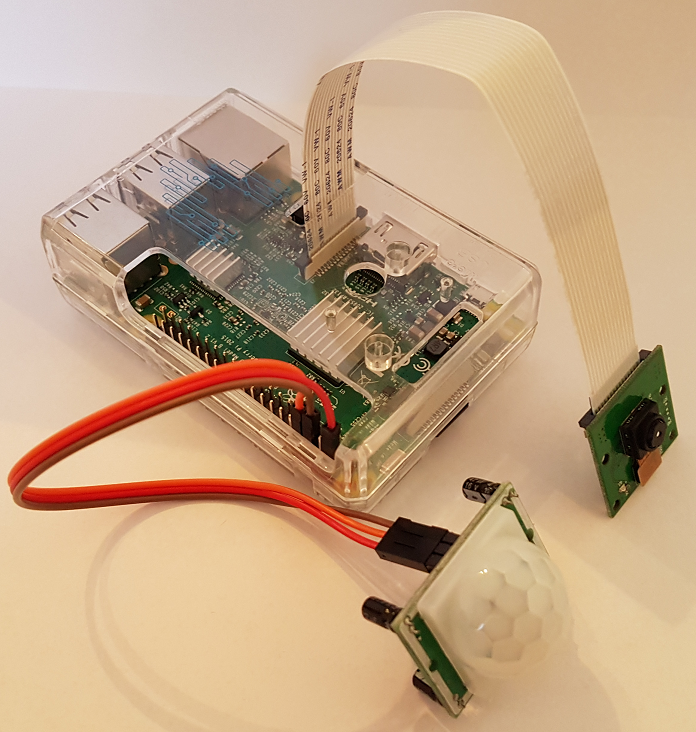
\includegraphics[scale=0.45]{\imageDir/rpisec-hardware-setup.png}
	\caption{Testaufbau der Applikation}
	\label{fig:image-hardware-setup}
\end{figure}
\ \newline
Wie in Abbildung \ref{fig:image-hardware-setup} zu ersichtlich ist, wurde die Kamera über CSI \emph{(Camera-Serial-Interface)}) und der Bewegungssensor über GPIO \emph{(General Purpose Input/Output)} an den \emph{Raspberry PI} angeschlossen.

\subsection{Betriebssysteme}
Dieser Abschnitt behandelt die verwendete Betriebssysteme für den \emph{Raspberry PI}. Die Applikation \emph{RPISec} wurde einerseits mit dem Betriebssystem \emph{hypriotos-rpi} und andererseits mit \emph{Raspian} realisiert. Das Betriebssystem \emph{hypriots} basiert auf \emph{Debian Jessie} und wird von dem \emph{OpenSource} Projekt \emph{hypriot}\footnote{\url{https://blog.hypriot.com/}} zur Verfügung gestellt wird. Das Ziel von \emph{hypriots} ist es ein Betriebssystem für \emph{Raspberry PI} zur Verfügung stellen, das bereits Docker vorinstalliert und betriebsbereit hat. Mit dem Betriebssystem \emph{Raspian} muss Docker selbst installiert, wobei Docker als Paket im \emph{Repository} zur Verfügung steht und daher sich die Installation als unkompliziert gestaltet.
\newline
\newline
Wenn Docker installiert und betriebsbereit ist, dann spielt es keine Rolle auf welchem Betriebssystem die Applikation \emph{RPISec} betrieben wird.
\newline
\newline
Da die Applikation \emph{RPISec} auf eine aktive Internetverbindung angewiesen ist, muss das Betriebssystem so konfiguriert werden, dass der \emph{Raspberry PI} entweder über \emph{Ethernet} oder \emph{Wlan} an ein Netzwerk angebunden ist, das Zugriff auf das Internet erlaubt. In einem produktiven Betrieb muss der \emph{Raspberry PI} über das Internet erreichbar sein, damit die mobilen \emph{Clients} Anfragen an die gehosteten \emph{Microservice} absetzen können.